\documentclass[10pt,a4paper,titlepage]{article}
\usepackage[utf8]{inputenc}
\usepackage[francais]{babel}
\usepackage[T1]{fontenc}
\usepackage{amsmath}
\usepackage{amsfonts}
\usepackage{amssymb}
\usepackage{graphicx}
\usepackage{wrapfig}
\usepackage{caption}
\usepackage{float}

\usepackage{color}   %May be necessary if you want to color links
\usepackage{hyperref}
\hypersetup{
    colorlinks=true, %set true if you want colored links
    linktoc=all,     %set to all if you want both sections and subsections linked
    linkcolor=blue,  %choose some color if you want links to stand out
}

\author{Valentin DESCHAINTRE, Théophile MADET}
\title{IN55\\Animation de personnage\\Rapport}

\begin{document}
\maketitle
\tableofcontents
\section{Intro}
Pour notre premier projet en synthèse d'image, nous avons choisi l'animation de personnage 3D. 
\par
En effet, en partant d'un personnage simpliste fait de formes géométriques, nous commencions avec des éléments que nous connaissions car nous les avions utilisés en TP. 
\par
De plus, effectuer un rendu de mouvement qui ait l'air naturel nous a semblé être un challenge intéressant. 
\section{Choix d'implémentation}
%Structure hiérarchique, classe BodyPart, angles simples, structure du main (pour l'ordre des push/popMatrix(), shader texture
Cette section présente les raisons qui ont menées aux choix de structure de notre projet.

\subsection{Hiérarchie de membres}
Chaque membre du corps possède un parent et un point d'accroche à ce parent. Sa position et son orientation dépendent de ceux du parent. Ainsi, on obtient un comportement similaire à celui d'une articulation du corps humain. 
\par
De plus, lors de l'analyse des mouvements du corps, il était plus simple d'étudier l'angle d'un membre par rapport à un autre que son angle absolu par rapport à une origine abstraite.  

\subsection{Classe BodyPart}
Étant donné que nous utilisons un langage objet, il était naturel de regrouper tous les membres du corps par une même classe. 
\begin{wrapfigure}{r}{.35\textwidth}
\centering
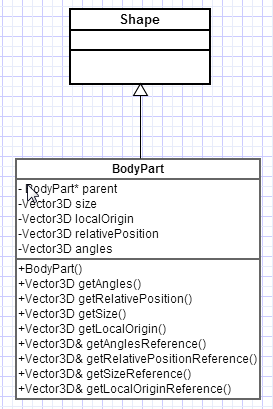
\includegraphics[width=.4\textwidth]{UML_Body_part.png}
\caption{Diagramme UML de la classe BodyPart}
\end{wrapfigure}
\par
Ainsi, chaque membre contient toutes les informations qui permettraient de l'afficher indépendamment\footnote{Ils sont toutefois affichés dans un ordre précis pour tirer parti du fonctionnement des pushMatrix() et popMatrix()}. 
\par
Pour pouvoir nous concentrer sur la qualité des animations, nous avons représenté toutes les parties du corps par des pavés (pas de sphère, pyramides...).

Les getter sont disponibles en deux version :
\begin{itemize}
	\item Retour par valeur, lorsqu'on veut simplement lire l'un des paramètres, pour l'affichage par exemple. Les fonctions \textit{getAngles}() et \textit{getRelativePosition}() donnent les valeurs absolues, c'est à dire prenant en compte la position et l'orientation du parent.
	\item Retour par référence, pour pouvoir modifier le paramètre demandé. Cela peut être vu comme contraire au modèle objet, mais c'est pour nous un équivalent de setter pratique pour nos fonctions d'animations. 
\end{itemize}

\subsection{Ordre d'affichage}
Nos \textit{BodyPart} ayant accès aux informations de leurs parents, nous aurions pu afficher chaque membre indépendamment. Nous avons tout de même choisi de tirer parti des méthodes \textit{push/popMatrix}(), ce qui permet à la méthode \textit{draw}() de \textit{BodyPart} de n'utiliser que ses propres paramètres. Ils n'ont pas besoin de lire ceux du parent.
\par
\begin{figure}[htbp]
\centering
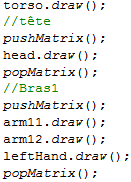
\includegraphics{exemple_code_matrix.png}
\caption{Exemple de code tirant parti de \textit{push/popMatrix}()}
\end{figure}
Voici un extrait de la fonction paintGL illustrant l'utilisation de cette structure. Le torse étant l'élément parent de la hiérarchie, il est affiché en premier. La tête, ensuite, se base sur la matrice du torse, mais n'influence pas les bras. La première partie du bras, à l'inverse, influence l'avant-bras, qui influence lui même la main.

\subsection{Représentation de l'animation}
Deux techniques différentes ont été utilisées pour décrire nos animations en code. Dans les deux cas la procédure a été similaire : 
\begin{itemize}
	\item Repérer les angles et positions importantes pour l'animation voulue. Par exemple pour le saut, l'angle du torse varie avec le temps, alors que ce n'est pas le cas pour la course et la marche.
	\item En se servant de dessins de référence\footnote{Exemple : http://www.animationresources.org/pics/pbanimation26-big.jpg}, ou en effectuant nous même les mouvements, noter à plusieurs instants les valeurs des positions et angles repérés lors de l'étape précédente.
	\item Déterminer la fonction mathématique passant par ces points clés.
\end{itemize}
Notre technique nous semble proche de l'animation par \textit{KeyFrames}, dans le sens où nous avons déterminé les instants clés des mouvements, puis avons interpolé les valeurs situées entre ces points clés. Toutefois, dans notre cas, nous avons effectué nous même l'interpolation, grâce à des outils mathématiques, de façon à pouvoir visualiser les fonctions et à les lisser, alors qu'une animation par \textit{KeyFrame} classique fera ce travail automatiquement.
\subsubsection{Animation de marche : fonctions sinus/cosinus}
L'animation de marche a été la plus simple des trois à mettre en place. En effet, une fois nos points clés placés, nous avons remarqué que les fonctions trigonométriques correspondaient bien pour toutes les valeurs repérées. Ainsi, toutes les valeurs sont fonctions de sinus ou de cosinus étirés, ralentis, décalés\dots
\subsubsection{Animation de course et de saut : interpolation de Lagrange}
Pour la course et le saut, il est vite apparu que les cosinus et sinus ne suffiraient pas, certains mouvements étant trop irréguliers. Notre idée a donc été d'utiliser l'interpolation de Lagrange apprise en \bsc{MT44} pour déterminer les fonctions correspondantes. Nous pensions ainsi obtenir directement les bonnes fonctions, quels que soit nos points de passage. Nous avons toutefois rencontré quelques difficultés, décrites dans la partie appropriée (\ref{interpolation}).

\subsection{Utilisation des shader de texture}

Afin de rendre l'ensemble plus agréable, nous avons décidé d'utiliser les shaders pour créer un environnement simple et donner au <<mannequin>> un effet <<bois>>. Pour ce faire nous avons créer un shader de texture et y avons associé 4 textures différentes : une texture de sol, de bois, de ciel et d'immeubles.
L'environnement est actuellement composé d'une longue rue borduré par des immeubles. 

\subsection{Bibliothèque GLM}
La bibliothèque GLM(OpenGL Mathematics) est une librairie C++ orienté pour les programme 3D. Elle permet d'utiliser une grande quantité de fonctionnalité et de classes de GLSL. Nous nous servons principalement des types vec3 et vec4 ainsi que de mat4 pour tout ce qui est gestion de la caméra.\\
Cette librairie n'a pas besoin d'être installé, il suffit d'inclure le fichier glm.hpp et de mettre le dossier glm-0.9.4.4 à la racine du projet.

\section{Difficultés rencontrées}
Durant ce projet nous avons rencontré différentes difficultés que nous allons tâcher de décrire ici, ainsi que les solutions que nous avons pu trouver ou non.
\subsection{Installation de QT}
Puisque nous avions commencé les TPs sur QT, nous avions déjà des bases dessus.\\

Notre première difficulté a été d'installer la bonne version de QT et de mingw pour que les TPs puissent être compilés sur nos machines.
Au début de l'installation nous ne comprenions pas pourquoi la compilation n'était pas possible (les messages d'erreurs n'étaient pas explicites).\\

Après avoir essayé différentes solutions trouvées sur le net nous avons utilisé un tutoriel du site du zéro qui répondait parfaitement à notre problématique. Il expliquait que les versions plus récentes avaient changé d'architecture et qu'il fallait donc rester sur la bonne version de QT et de mingw.\\
Ce tutoriel guidait dans l'installation et la configuration de la bonne version de QT et de mingw et fournissait les fichiers associés. L'installation de la bonne version nous a permis de nous baser sur le framework des TPs.


\subsection{Interpolation incorrecte}
\label{interpolation}
L'avantage de cet outil (l'interpolation de Lagrange) est qu'il propose des fonctions lissées, donnant un aspect plus naturel aux mouvement. Toutefois, lorsqu'il est utilisé avec beaucoup de points de passages, il donne des fonctions très complexes avec des écarts très grands, ne donnant pas le résultat attendu.
\par
Nous avons donc au final décomposé nos animations en sections regroupant 3 ou 4 points de passage au maximum. Les liaisons sont parfois un peu abruptes mais par tâtonnement, grâce à des traceurs de graphes de fonctions, nous avons pu limiter les cassures. 
\par
Voici un exemple de composition de fonctions interpolées et de cosinus. L'animation se déroule sur 6 unités de temps, et représente l'angle de la cuisse par rapport au torse lors du saut, l'angle zéro étant la position debout. La fonction bleue est utilisée de 0 à 2, puis la rouge de 2 à 4 et la verte de 4 à 6.
\begin{figure}[H]
\centering
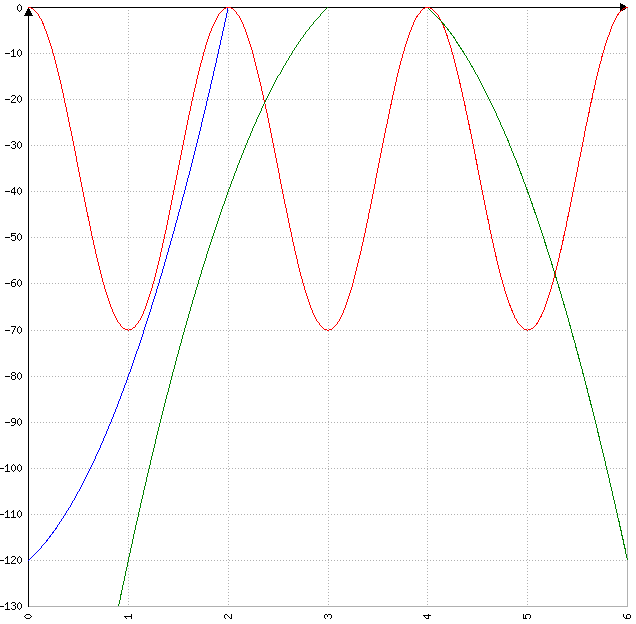
\includegraphics[width=.5\textwidth]{exemple_interpolation.png}
\caption{Exemple de fonctions utilisées pour l'animation}
\end{figure}


\subsection{Implémentation de la caméra}
Au vu de la difficulté que nous avons rencontré lors de l'implémentation de la caméra en TP, nous avons décidé d'implémenter une caméra plus simple.\\
Elle permet également des mouvements libres  mais n'utilise pas les quaternions. Ce choix implique un risque de "Gimbal Lock" dans le cas où deux plans se trouveraient coplanaires, mais compte tenu du temps limité pour le projet, et de la charge de travail du reste des UVs nous avons préféré implémenter une première caméra fonctionnelle.

Celle-ci permet de se déplacer, de tourner la tête, de monter et de descendre ainsi que de faire tourner la scène.

Pour permettre de tels déplacement nous avons utilisé les matrices projectives vu en cours et TD associés à un double changement de repère. Cela permet de centrer les rotations à la position de la caméra afin de donner une impression de "tourner la tête".

La caméra utilise des isométries vectorielle plutôt qu'affine. Ceci permet de normer les vecteurs et d'avoir toujours le point à regarder à une distance raisonnable de la caméra.\\ 
Pour les déplacements latéraux il nous a suffit de calculer le vecteur normé entre la position de la caméra et le point observé et d'y appliquer une rotation de $\pi/2$ ou -$\pi/2$ pour obtenir le mouvement souhaité à un facteur de vitesse près.

\subsection{Distance d'affichage}

Pour notre rendu nous avons choisi d'avoir un humain de taille "normale", les unités que nous avons choisies étant 1/10cm. De ce fait lors de la création d'une scène autour de l'animation, nous avons du faire face au non affichage des éléments à une distance de plus de 40 unités de la caméra.\\

Nous avons donc modifié le framework afin que la limitation se fasse après 1000 unités. Ce qui nous permet d'obtenir cette longue "cour intérieur".

\subsection{Position du corps}
Dans notre hiérarchie de membres, le torse est le parent : c'est lui qui sert de référence aux autres. C'est ce qui nous semblait le plus naturel lors de l'écriture de nos animations. 
\par
Toutefois, cela pose un problème : lorsque le pantin saute ou marche, le torse monte ou descend, et les jambes se plient et se déplient. Comment alors s'assurer que les pieds touchent le sol lorsqu'il le faut? 
\par
Nous aurions pu changer de parent pour l'un des pieds, mais ce n'est pas très naturel. Nous avons donc au final réglé nos distances par tâtonnement, avec parfois un peu de géométrie basique, puisque nous connaissions toutes les longueurs nécessaires. 


\subsection{Luminosité}
Nous avons souhaité intégrer la gestion de la luminosité à notre projet, cependant malgré nos essais nous n'avons pas réussi à obtenir un résultat satisfaisant. Nous avons donc préféré laisser la luminosité par défaut.  

\subsection{Extraction d'exécutable}
Lors de la compilation un fichier .exe est fourni. Nous avons cherché à rendre ce .exe exécutable sans avoir besoin d'autre fichiers que les shaders et les images.\\
Après ajout de quelques .dll nous sommes arrivé à un exécutable fonctionnel sur nos deux ordinateurs.\\
Nous nous sommes cependant aperçu qu'en le lançant sur une autre machine la fenêtre apparaissait noir. Nous n'avons pas pu déterminer la raison de ce problème. Il est cependant toujours possible de lancer le programme via QT, le soucis ne nous a donc pas paru critique.

\section{Captures d'écran}
\begin{figure}[H]
\centering
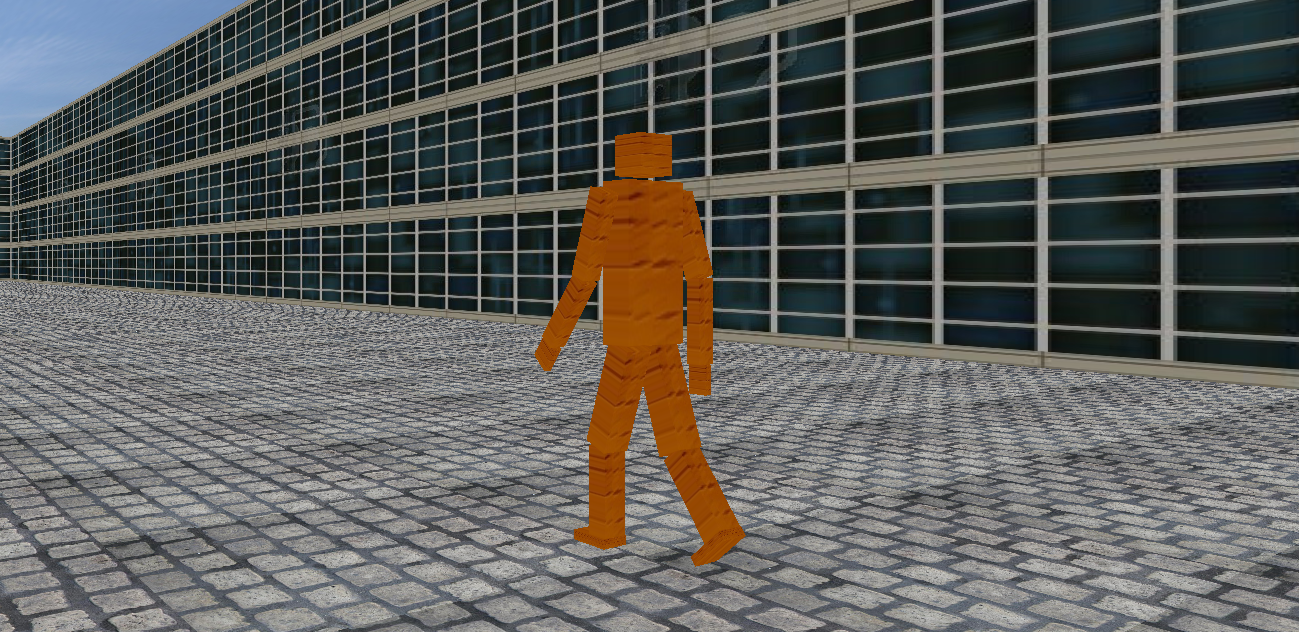
\includegraphics[width=1\textwidth]{init.png}
\caption{Position du base du mannequin}
\end{figure}

\begin{figure}[H]
\centering
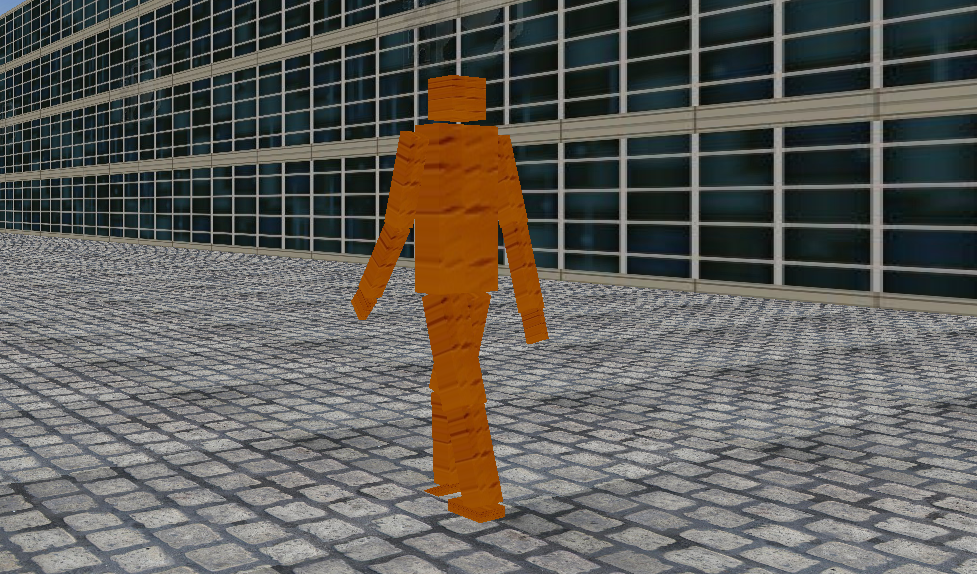
\includegraphics[width=1\textwidth]{walk.png}
\caption{Marche}
\end{figure}

\begin{figure}[H]
\centering
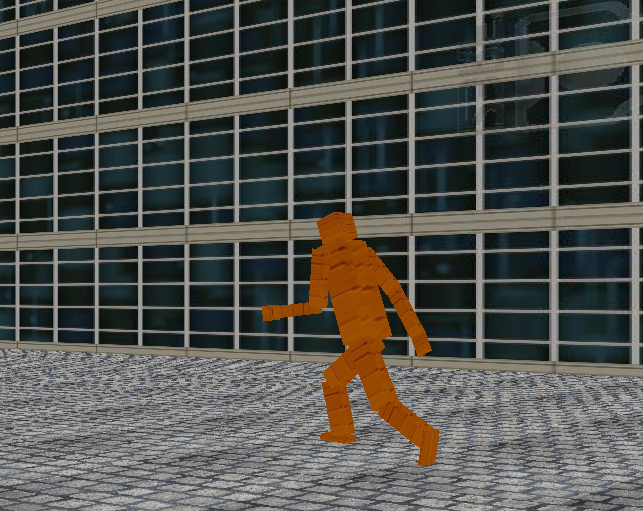
\includegraphics[width=1\textwidth]{run.png}
\caption{Course}
\end{figure}

\begin{figure}[H]
\centering
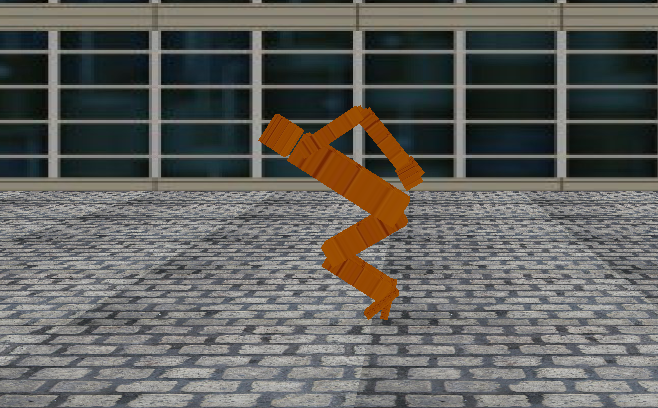
\includegraphics[width=1\textwidth]{saut1.png}
\caption{Saut (amorce)}
\end{figure}

\begin{figure}[H]
\centering
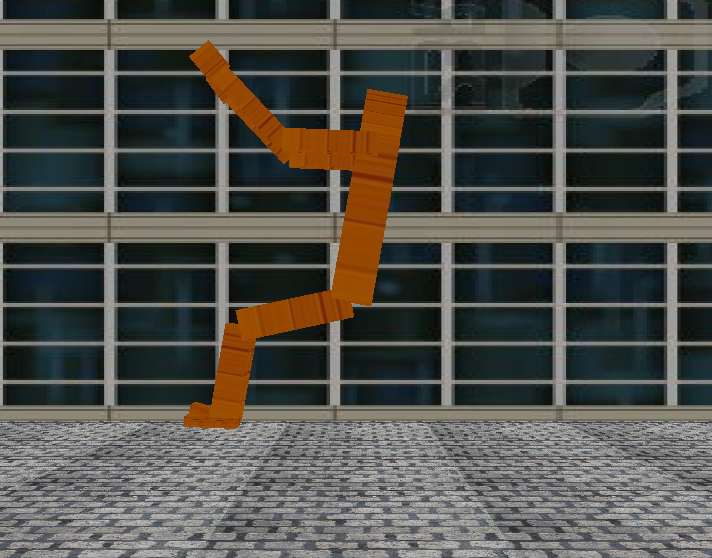
\includegraphics[width=1\textwidth]{saut2.png}
\caption{Saut (en l'air)}
\end{figure}

\section{Guide d'utilisation}
Voici les différents raccourcis utilisés pour manipuler le programme :
\begin{description}
	\item[A,E :] Incrémente ou décrémente l'index de l'animation. Les index utilisés sont : 
	\begin{description}
		\item[0 :]pas de mouvement,
		\item[1 :]marche,
		\item[2 :]course,
		\item[3 :]saut.
	\end{description}
	\item[Z,Q,S,D :] déplace la caméra vers l'avant, gauche, arrière, droite respectivement.
	\item[$\leftarrow,\uparrow,\downarrow,\rightarrow$ :]fait tourner la scène autours de son origine absolue.
	\item[Souris :] Maintenir un clic et déplacer la souris fera tourner la caméra dans la direction demandée.
\end{description}

\section{Améliorations possibles}
Au cours de ce projet, nous avons surtout cherché à mettre en place des techniques (animation, shader\dots), et à s'assurer qu'elles étaient fonctionnelles. Elle ne sont toutefois pas poussées à leur maximum, laissant de nombreuses possibilités d'amélioration.
\begin{itemize}

\item Un shader de gestion de la lumière pourrait être ajouté, pour un rendu plus réaliste.

\item Des textures plus intéressantes pourraient être utilisées, notamment pour faire du pantin un personnage humain. Nous avons commencé à nous y intéressé, d'où les textures de Solid Snake dans le dossier img.

\item Toujours pour améliorer le personnage, il serait possible de détailler plus les différents membres. Il serait également possible d'ajouter des volumes paramétriques aux articulations pour maintenir une liaison constante entre les membres.

\item En jouant deux animations à la fois et en affectant un poids à chacune, les vertices seraient alors une moyenne pondérée des deux animations. Cela donnerait des transitions lissées entre deux animations plutôt qu'une cassure.

\end{itemize}
\section{Conclusion}
En conclusion, nous pouvons dire que ce projet nous a permis de comprendre comment fonctionnait l'animation 3D ainsi que la représentation d'une scène. Avec les TPs, il aura été notre introduction au monde d'OpenGL.
\par
\'Etant tous les deux assidus joueurs de jeux vidéos, nous avions souvent entendu parler de shader. Nous savons aujourd'hui ce qu'ils sont et avons pu expérimenter leurs effets. 

Le projet nous a également permis de mettre en pratique les outils vu en cours et TD, notamment les matrices projectives ou les techniques d'animation et de texture.
\end{document}